\subsection{Prueba de rendimiento}
Esta prueba se realiza una vez que hechas las modificaciones como producto de las pruebas unitarias, de integración y de sistema.
\subsubsection{Objetivo de la prueba}
Verificar el uso del GPU, el nivel de bateria del telefono que utiliza y la temperatura del telefono mientras la aplicación este funcionando. 
\subsubsection{Herramientas utilizadas durante la prueba}
Opciones de desarrollador del telefono Huawei TAG-L13 y \textit{Baterry Doctor}.
\subsubsection{Aplicación de la prueba}
Para esta prueba se debe de instalar la apk del juego en el dispositivo, activar las 
opciones de desarrollador e instalar la aplicación \textit{Baterry Doctor}.  Una vez 
hecho esto se juega el juego y se mide el desempeño desde el telefono. En las figura 
\ref{fig:GPUHuawei} se muestra el uso del GPU en distintos momentos de la partidad.
\\
\par
\begin{figure}
  \centering
  
   \subfigure[Uso del GPU desde el menú principal.] {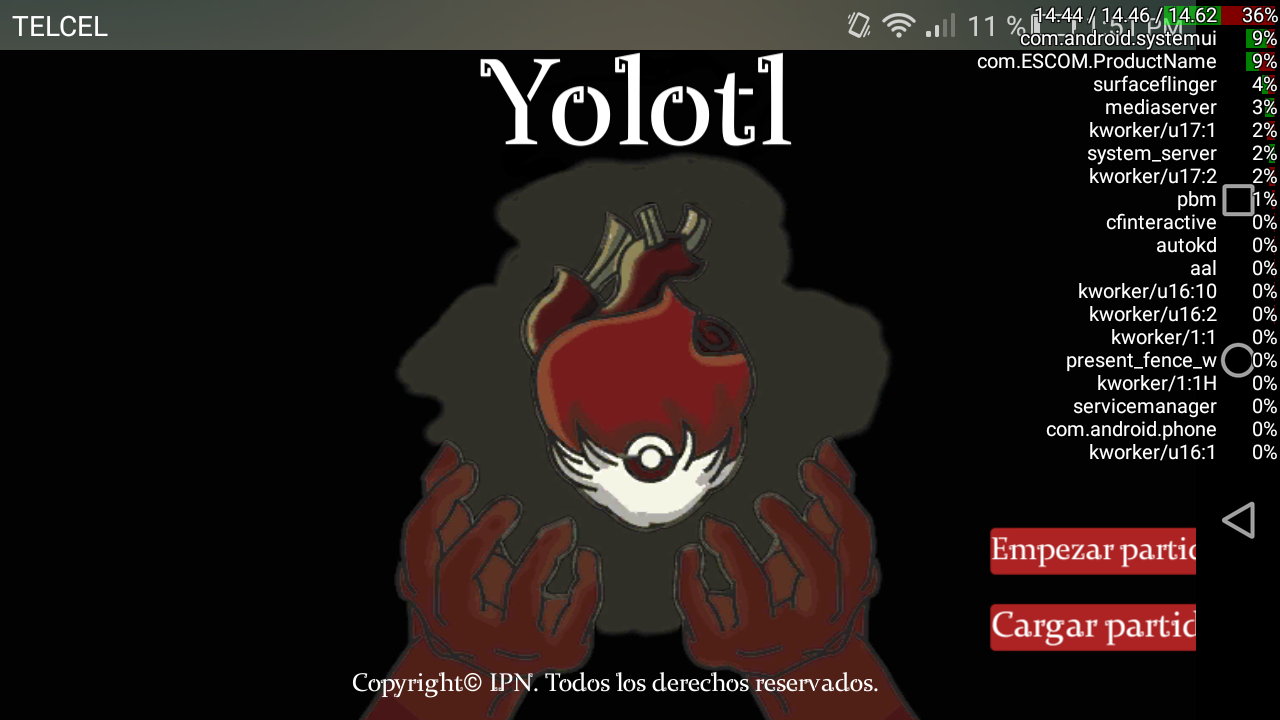
\includegraphics[width=0.4 \textwidth]{04ResultadosObetnidos/imagenes/rendimiento01.png}}
   
   \subfigure[Uso del GPU desde el menú de selección de nivel.] {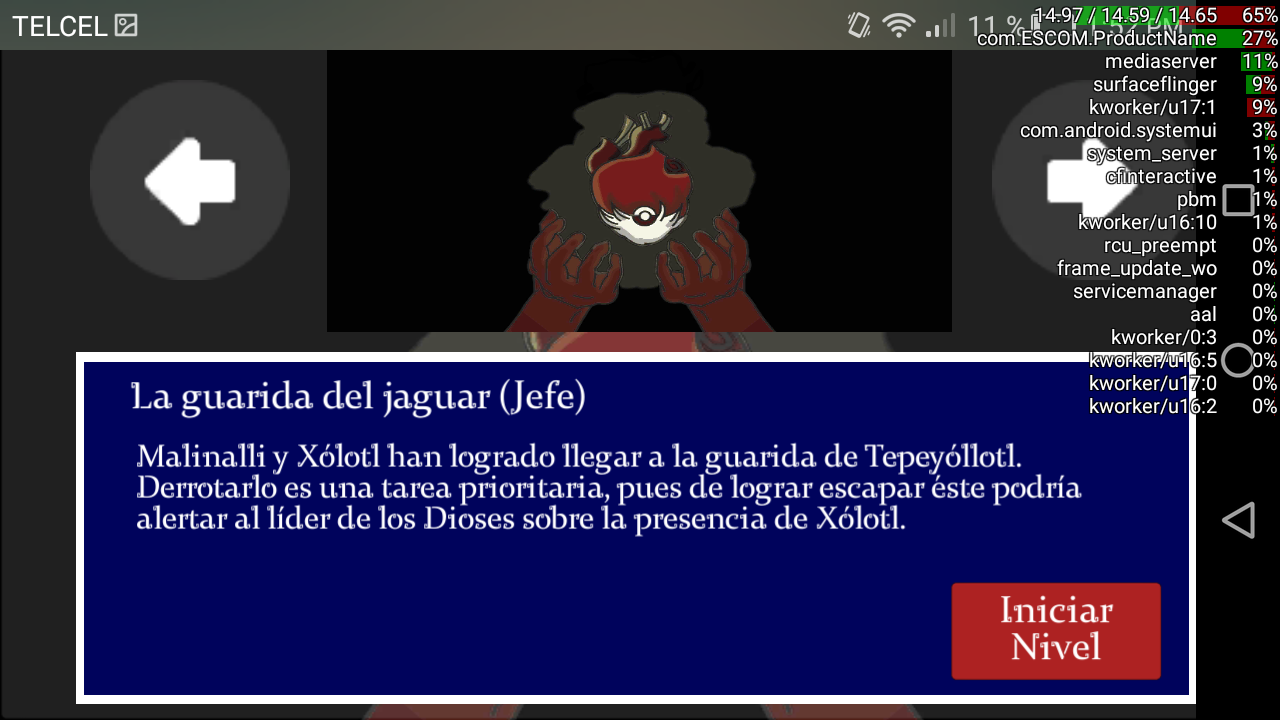
\includegraphics[width=0.4 \textwidth]{04ResultadosObetnidos/imagenes/rendimiento02.png}}
   
   \subfigure[Uso del GPU desde una cinemática.] {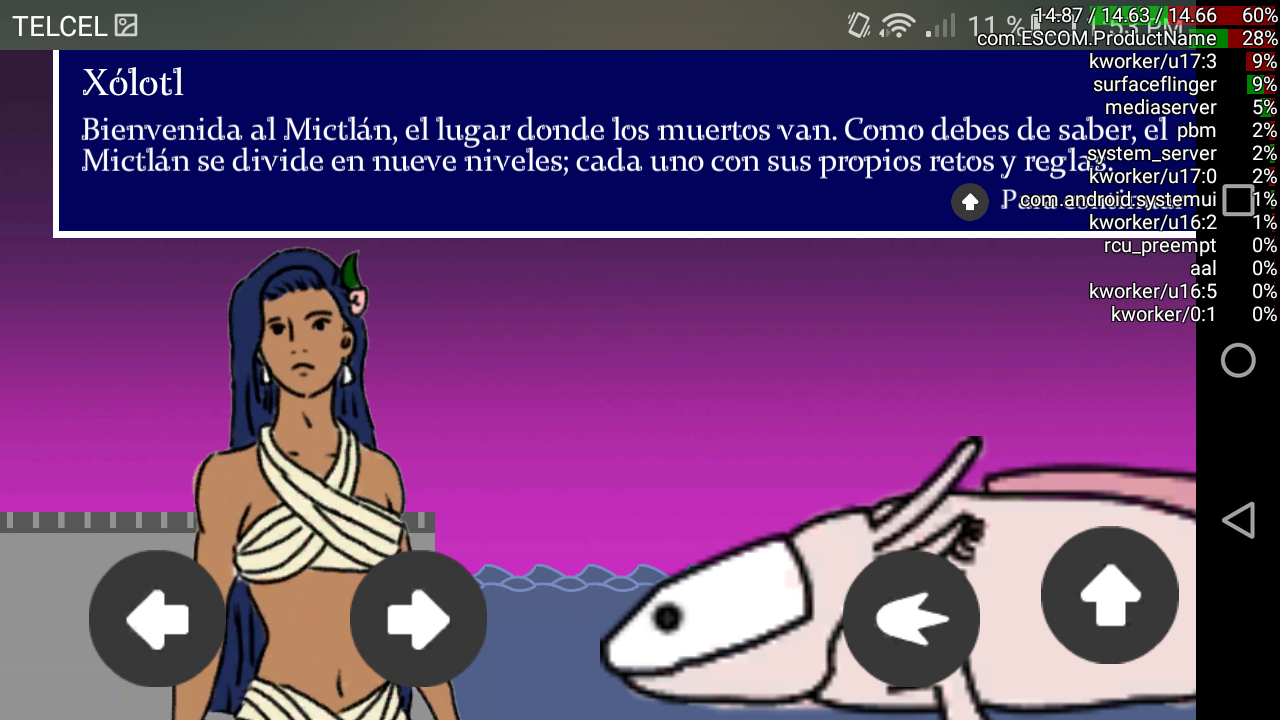
\includegraphics[width=0.4 \textwidth]{04ResultadosObetnidos/imagenes/rendimiento03.png}}
   
   \subfigure[Uso del GPU desde un nivel de plataforma.] {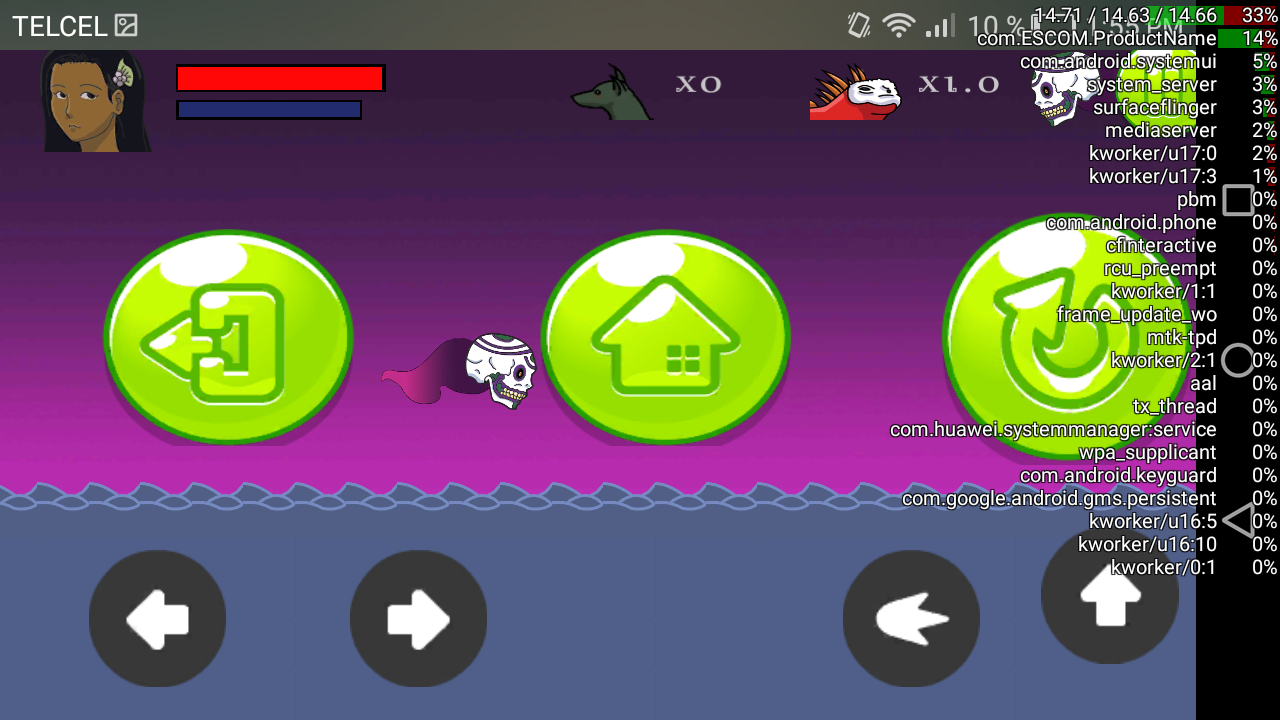
\includegraphics[width=0.4 \textwidth]{04ResultadosObetnidos/imagenes/rendimiento05.png}}
   
   \subfigure[Uso del GPU desde un nivel de jefe.] {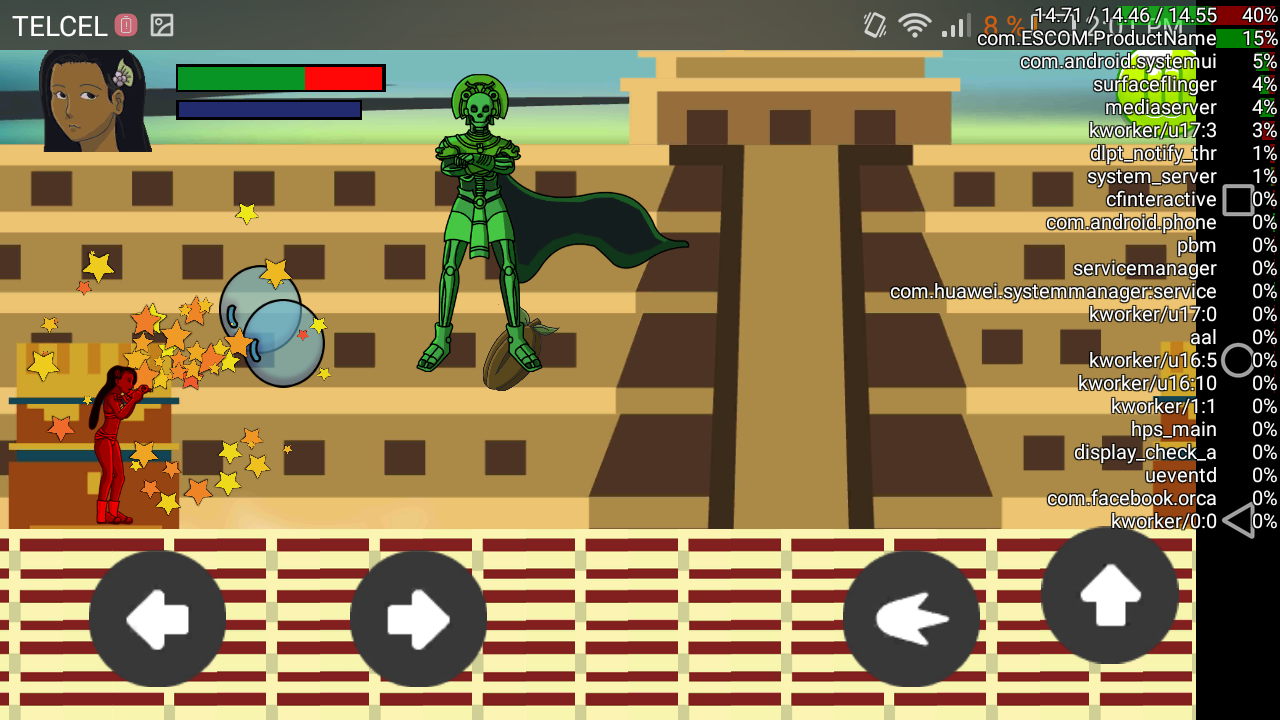
\includegraphics[width=0.4 \textwidth]{04ResultadosObetnidos/imagenes/rendimiento10.png}}
   
  \caption{Resultados del rendimiento del GPU del dispositivo Huawei}
  \label{fig:GPUHuawei}
\end{figure} 

\subsubsection{Conclusiones de la prueba}
De esta medición del desempeño del GPU se puede observar que la aplicacion utiliza un minimo del 9\% del GPU y ahasta un maximo del casi el 30\%. Por su parte la temperatura del telefono no se ve afectada manera significativa y en promedio utiliza un 10\% de la batería. Estas cifras son buenas si se considera que otras aplicaciones como \textit{Messenger} de \textit{Facebook} llega a utilizar el 50.6\% del GPU y casi el 60\% de la bateria del telefono, ver figura . 